% EE463 cheat sheet (midterm): one A4 page, single side.
% Scope: everything up to the end of INDUCTOR magnetic design + labs (Exp 1, Exp 2).
% No DCM. Not included: Cuk, SEPIC, Zeta, bridge converters, four-quadrant, transformer design.
% Circuit figures are given in the exam, so only waveform sketches are here.
% Only PAGE 1 is printed: check the page count after every edit.
\documentclass{article}
\usepackage{fix-cm}
\usepackage[T1]{fontenc}
\usepackage{lmodern}
\usepackage[a4paper,left=5mm,right=5mm,top=5mm,bottom=5mm]{geometry}
\usepackage{amsmath,amssymb,multicol,array}
\usepackage{xcolor}
\usepackage{tikz}
\usetikzlibrary{arrows.meta}
\pagestyle{empty}
\setlength{\parindent}{0pt}
\setlength{\parskip}{0.8pt}
\setlength{\columnsep}{3mm}
\setlength{\columnseprule}{0.4pt}
\setlength{\fboxsep}{0.8pt}
\newcommand{\hd}[1]{\par\vspace{1.5pt}\fbox{\parbox{\dimexpr\linewidth-2\fboxsep-0.8pt}{\textbf{#1}}}\par\vspace{0.8pt}}
\newcommand{\sh}[1]{\textbf{#1:}\ }
\newcommand{\nt}[1]{#1}
\thinmuskip=1.5mu \medmuskip=2mu \thickmuskip=2.5mu

\begin{document}
\fontsize{8.8}{10.03}\selectfont
\setlength{\abovedisplayskip}{0pt}\setlength{\belowdisplayskip}{0pt}
\setlength{\abovedisplayshortskip}{0pt}\setlength{\belowdisplayshortskip}{0pt}
\begin{multicols*}{3}
\raggedright
\textbf{\fontsize{8.5}{9.5}\selectfont EE463 Cheat Sheet} {\fontsize{7}{8}\selectfont\nt{by Yi\u{g}it Emre Demiral}}\\
\nt{$D$: duty cycle, $T_s=1/f_s$, $V_s$: rms source voltage, $\omega=2\pi f$}

%=========================================================
\hd{Waveform Quality}
RMS: $I_{rms}=\sqrt{\frac1T\int_0^T i^2\,dt}=\sqrt{I_{dc}^2+I_1^2+I_2^2+\dots}$\\
THD $=\dfrac{\sqrt{I_{rms}^2-I_1^2}}{I_1}$ \quad ($I_1$: rms of fundamental)\\
Distortion factor: DF $=\dfrac{I_1}{I_{rms}}=\dfrac{1}{\sqrt{1+\text{THD}^2}}$\\
Displacement PF: DPF $=\cos\phi_1$ \nt{($\phi_1$: angle between $v_s$ and $i_1$)}\\
Power factor: PF $=\dfrac{P}{V_sI_{rms}}=$ DF $\times$ DPF \quad Crest factor: CF $=\dfrac{I_{peak}}{I_{rms}}$\\
\sh{Useful RMS}
pulse of height $I$ for $DT$: $I\sqrt D$ \quad triangle $0\to I_p$: $I_p/\sqrt3$\\
DC $I$ + triangle ripple $\Delta i$ (p-p): $\sqrt{I^2+\Delta i^2/12}$\\
\sh{Fourier} $a_h=\frac2T\int_0^T f\cos(h\omega t)dt$,\ $b_h=\frac2T\int_0^T f\sin(h\omega t)dt$\\
Square wave $\pm A$: peak of $h$-th harmonic $=\frac{4A}{h\pi}$ ($h$ odd)\\
\sh{Steady state} avg.\ $v_L=0$ (volt-sec balance), avg.\ $i_C=0$ (amp-sec balance)

%=========================================================
\hd{Single-Phase Diode Rectifiers}
\sh{Half-wave, R load} $V_{avg}=\frac{\sqrt2V_s}{\pi}=0.45V_s$\\
\sh{Half-wave, RL load} conducts past $\pi$ until $i=0$ at $\beta$:\\
$V_{avg}=\frac{\sqrt2V_s}{2\pi}(1-\cos\beta)$\\
\sh{With back-EMF $E$} diode on when $v_s>E$: starts at $\theta_b=\sin^{-1}\frac{E}{\sqrt2V_s}$; $i$ peaks at $\pi-\theta_b$; stops at $\theta_f$ where
$\int_{\theta_b}^{\theta_f}(\sqrt2V_s\sin\theta-E)\,d\theta=0$ (equal areas)\\
\sh{Full bridge, no $L_s$} $V_d=\frac{2\sqrt2}{\pi}V_s=0.9V_s$\\
If $I_d$ constant: $i_s$ is a square wave $\pm I_d$\\
$I_s=I_d$, $I_{s1}=0.9I_d$, $I_{sh}=I_{s1}/h$ ($h$=3,5,7..)\\
DPF $=1$, PF $=0.9$, THD $=48.4\%$\\
\sh{Full bridge with $L_s$ (commutation)} $i_s$ needs time $u$ to go from $-I_d$ to $+I_d$, $v_d=0$ during $u$:\\
$\cos u=1-\dfrac{2\omega L_sI_d}{\sqrt2V_s}$, \quad $V_d=0.9V_s-\dfrac{2\omega L_sI_d}{\pi}$

\par\noindent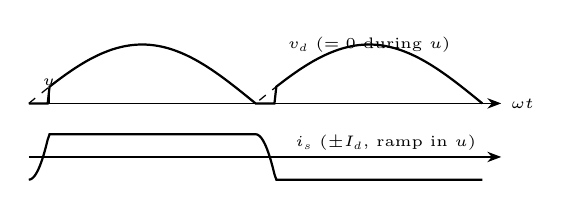
\begin{tikzpicture}[baseline=(current bounding box.south),x=9.6mm,y=3.4mm,font=\fontsize{5.5}{6}\selectfont,line width=0.45pt,>=Stealth]
\draw[->,black] (0,0)--(6.25,0) node[right,black]{$\omega t$};
\draw[dashed,black] plot coordinates{(0.000,0.000) (0.025,0.058) (0.050,0.115) (0.075,0.173) (0.100,0.230) (0.125,0.287) (0.150,0.344) (0.175,0.401) (0.200,0.457) (0.225,0.514) (0.250,0.569) (0.275,0.625) (0.300,0.680) (0.325,0.734) (0.350,0.788) (0.375,0.842) (0.400,0.895) (0.425,0.947) (0.450,0.999) (0.475,1.050) (0.500,1.100) (0.525,1.149) (0.550,1.198) (0.575,1.246) (0.600,1.293) (0.625,1.339) (0.650,1.385) (0.675,1.429) (0.700,1.472) (0.725,1.514) (0.750,1.556) (0.775,1.596) (0.800,1.635) (0.825,1.673) (0.850,1.710) (0.875,1.745) (0.900,1.780) (0.925,1.813) (0.950,1.845) (0.975,1.876) (1.000,1.905) (1.025,1.933) (1.050,1.960) (1.075,1.986) (1.100,2.010) (1.125,2.033) (1.150,2.054) (1.175,2.074) (1.200,2.092) (1.225,2.109) (1.250,2.125) (1.275,2.139) (1.300,2.152) (1.325,2.163) (1.350,2.173) (1.375,2.181) (1.400,2.188) (1.425,2.193) (1.450,2.197) (1.475,2.199) (1.500,2.200) (1.525,2.199) (1.550,2.197) (1.575,2.193) (1.600,2.188) (1.625,2.181) (1.650,2.173) (1.675,2.163) (1.700,2.152) (1.725,2.139) (1.750,2.125) (1.775,2.109) (1.800,2.092) (1.825,2.074) (1.850,2.054) (1.875,2.033) (1.900,2.010) (1.925,1.986) (1.950,1.960) (1.975,1.933) (2.000,1.905) (2.025,1.876) (2.050,1.845) (2.075,1.813) (2.100,1.780) (2.125,1.745) (2.150,1.710) (2.175,1.673) (2.200,1.635) (2.225,1.596) (2.250,1.556) (2.275,1.514) (2.300,1.472) (2.325,1.429) (2.350,1.385) (2.375,1.339) (2.400,1.293) (2.425,1.246) (2.450,1.198) (2.475,1.149) (2.500,1.100) (2.525,1.050) (2.550,0.999) (2.575,0.947) (2.600,0.895) (2.625,0.842) (2.650,0.788) (2.675,0.734) (2.700,0.680) (2.725,0.625) (2.750,0.569) (2.775,0.514) (2.800,0.457) (2.825,0.401) (2.850,0.344) (2.875,0.287) (2.900,0.230) (2.925,0.173) (2.950,0.115) (2.975,0.058) (3.000,0.000) (3.025,0.058) (3.050,0.115) (3.075,0.173) (3.100,0.230) (3.125,0.287) (3.150,0.344) (3.175,0.401) (3.200,0.457) (3.225,0.514) (3.250,0.569) (3.275,0.625) (3.300,0.680) (3.325,0.734) (3.350,0.788) (3.375,0.842) (3.400,0.895) (3.425,0.947) (3.450,0.999) (3.475,1.050) (3.500,1.100) (3.525,1.149) (3.550,1.198) (3.575,1.246) (3.600,1.293) (3.625,1.339) (3.650,1.385) (3.675,1.429) (3.700,1.472) (3.725,1.514) (3.750,1.556) (3.775,1.596) (3.800,1.635) (3.825,1.673) (3.850,1.710) (3.875,1.745) (3.900,1.780) (3.925,1.813) (3.950,1.845) (3.975,1.876) (4.000,1.905) (4.025,1.933) (4.050,1.960) (4.075,1.986) (4.100,2.010) (4.125,2.033) (4.150,2.054) (4.175,2.074) (4.200,2.092) (4.225,2.109) (4.250,2.125) (4.275,2.139) (4.300,2.152) (4.325,2.163) (4.350,2.173) (4.375,2.181) (4.400,2.188) (4.425,2.193) (4.450,2.197) (4.475,2.199) (4.500,2.200) (4.525,2.199) (4.550,2.197) (4.575,2.193) (4.600,2.188) (4.625,2.181) (4.650,2.173) (4.675,2.163) (4.700,2.152) (4.725,2.139) (4.750,2.125) (4.775,2.109) (4.800,2.092) (4.825,2.074) (4.850,2.054) (4.875,2.033) (4.900,2.010) (4.925,1.986) (4.950,1.960) (4.975,1.933) (5.000,1.905) (5.025,1.876) (5.050,1.845) (5.075,1.813) (5.100,1.780) (5.125,1.745) (5.150,1.710) (5.175,1.673) (5.200,1.635) (5.225,1.596) (5.250,1.556) (5.275,1.514) (5.300,1.472) (5.325,1.429) (5.350,1.385) (5.375,1.339) (5.400,1.293) (5.425,1.246) (5.450,1.198) (5.475,1.149) (5.500,1.100) (5.525,1.050) (5.550,0.999) (5.575,0.947) (5.600,0.895) (5.625,0.842) (5.650,0.788) (5.675,0.734) (5.700,0.680) (5.725,0.625) (5.750,0.569) (5.775,0.514) (5.800,0.457) (5.825,0.401) (5.850,0.344) (5.875,0.287) (5.900,0.230) (5.925,0.173) (5.950,0.115) (5.975,0.058) (6.000,0.000)};
\draw[thick] plot coordinates{(0.000,0.000) (0.025,0.000) (0.050,0.000) (0.075,0.000) (0.100,0.000) (0.125,0.000) (0.150,0.000) (0.175,0.000) (0.200,0.000) (0.225,0.000) (0.250,0.000) (0.275,0.625) (0.300,0.680) (0.325,0.734) (0.350,0.788) (0.375,0.842) (0.400,0.895) (0.425,0.947) (0.450,0.999) (0.475,1.050) (0.500,1.100) (0.525,1.149) (0.550,1.198) (0.575,1.246) (0.600,1.293) (0.625,1.339) (0.650,1.385) (0.675,1.429) (0.700,1.472) (0.725,1.514) (0.750,1.556) (0.775,1.596) (0.800,1.635) (0.825,1.673) (0.850,1.710) (0.875,1.745) (0.900,1.780) (0.925,1.813) (0.950,1.845) (0.975,1.876) (1.000,1.905) (1.025,1.933) (1.050,1.960) (1.075,1.986) (1.100,2.010) (1.125,2.033) (1.150,2.054) (1.175,2.074) (1.200,2.092) (1.225,2.109) (1.250,2.125) (1.275,2.139) (1.300,2.152) (1.325,2.163) (1.350,2.173) (1.375,2.181) (1.400,2.188) (1.425,2.193) (1.450,2.197) (1.475,2.199) (1.500,2.200) (1.525,2.199) (1.550,2.197) (1.575,2.193) (1.600,2.188) (1.625,2.181) (1.650,2.173) (1.675,2.163) (1.700,2.152) (1.725,2.139) (1.750,2.125) (1.775,2.109) (1.800,2.092) (1.825,2.074) (1.850,2.054) (1.875,2.033) (1.900,2.010) (1.925,1.986) (1.950,1.960) (1.975,1.933) (2.000,1.905) (2.025,1.876) (2.050,1.845) (2.075,1.813) (2.100,1.780) (2.125,1.745) (2.150,1.710) (2.175,1.673) (2.200,1.635) (2.225,1.596) (2.250,1.556) (2.275,1.514) (2.300,1.472) (2.325,1.429) (2.350,1.385) (2.375,1.339) (2.400,1.293) (2.425,1.246) (2.450,1.198) (2.475,1.149) (2.500,1.100) (2.525,1.050) (2.550,0.999) (2.575,0.947) (2.600,0.895) (2.625,0.842) (2.650,0.788) (2.675,0.734) (2.700,0.680) (2.725,0.625) (2.750,0.569) (2.775,0.514) (2.800,0.457) (2.825,0.401) (2.850,0.344) (2.875,0.287) (2.900,0.230) (2.925,0.173) (2.950,0.115) (2.975,0.058) (3.000,0.000) (3.025,0.000) (3.050,0.000) (3.075,0.000) (3.100,0.000) (3.125,0.000) (3.150,0.000) (3.175,0.000) (3.200,0.000) (3.225,0.000) (3.250,0.000) (3.275,0.625) (3.300,0.680) (3.325,0.734) (3.350,0.788) (3.375,0.842) (3.400,0.895) (3.425,0.947) (3.450,0.999) (3.475,1.050) (3.500,1.100) (3.525,1.149) (3.550,1.198) (3.575,1.246) (3.600,1.293) (3.625,1.339) (3.650,1.385) (3.675,1.429) (3.700,1.472) (3.725,1.514) (3.750,1.556) (3.775,1.596) (3.800,1.635) (3.825,1.673) (3.850,1.710) (3.875,1.745) (3.900,1.780) (3.925,1.813) (3.950,1.845) (3.975,1.876) (4.000,1.905) (4.025,1.933) (4.050,1.960) (4.075,1.986) (4.100,2.010) (4.125,2.033) (4.150,2.054) (4.175,2.074) (4.200,2.092) (4.225,2.109) (4.250,2.125) (4.275,2.139) (4.300,2.152) (4.325,2.163) (4.350,2.173) (4.375,2.181) (4.400,2.188) (4.425,2.193) (4.450,2.197) (4.475,2.199) (4.500,2.200) (4.525,2.199) (4.550,2.197) (4.575,2.193) (4.600,2.188) (4.625,2.181) (4.650,2.173) (4.675,2.163) (4.700,2.152) (4.725,2.139) (4.750,2.125) (4.775,2.109) (4.800,2.092) (4.825,2.074) (4.850,2.054) (4.875,2.033) (4.900,2.010) (4.925,1.986) (4.950,1.960) (4.975,1.933) (5.000,1.905) (5.025,1.876) (5.050,1.845) (5.075,1.813) (5.100,1.780) (5.125,1.745) (5.150,1.710) (5.175,1.673) (5.200,1.635) (5.225,1.596) (5.250,1.556) (5.275,1.514) (5.300,1.472) (5.325,1.429) (5.350,1.385) (5.375,1.339) (5.400,1.293) (5.425,1.246) (5.450,1.198) (5.475,1.149) (5.500,1.100) (5.525,1.050) (5.550,0.999) (5.575,0.947) (5.600,0.895) (5.625,0.842) (5.650,0.788) (5.675,0.734) (5.700,0.680) (5.725,0.625) (5.750,0.569) (5.775,0.514) (5.800,0.457) (5.825,0.401) (5.850,0.344) (5.875,0.287) (5.900,0.230) (5.925,0.173) (5.950,0.115) (5.975,0.058) (6.000,0.000)};
\draw[->,black] (0,-2.0)--(6.25,-2.0) node[right,black]{};
\draw[thick,black] plot coordinates{(0.000,-2.850) (0.025,-2.835) (0.050,-2.790) (0.075,-2.715) (0.100,-2.610) (0.125,-2.475) (0.150,-2.310) (0.175,-2.115) (0.200,-1.891) (0.225,-1.637) (0.250,-1.355) (0.275,-1.150) (0.300,-1.150) (0.325,-1.150) (0.350,-1.150) (0.375,-1.150) (0.400,-1.150) (0.425,-1.150) (0.450,-1.150) (0.475,-1.150) (0.500,-1.150) (0.525,-1.150) (0.550,-1.150) (0.575,-1.150) (0.600,-1.150) (0.625,-1.150) (0.650,-1.150) (0.675,-1.150) (0.700,-1.150) (0.725,-1.150) (0.750,-1.150) (0.775,-1.150) (0.800,-1.150) (0.825,-1.150) (0.850,-1.150) (0.875,-1.150) (0.900,-1.150) (0.925,-1.150) (0.950,-1.150) (0.975,-1.150) (1.000,-1.150) (1.025,-1.150) (1.050,-1.150) (1.075,-1.150) (1.100,-1.150) (1.125,-1.150) (1.150,-1.150) (1.175,-1.150) (1.200,-1.150) (1.225,-1.150) (1.250,-1.150) (1.275,-1.150) (1.300,-1.150) (1.325,-1.150) (1.350,-1.150) (1.375,-1.150) (1.400,-1.150) (1.425,-1.150) (1.450,-1.150) (1.475,-1.150) (1.500,-1.150) (1.525,-1.150) (1.550,-1.150) (1.575,-1.150) (1.600,-1.150) (1.625,-1.150) (1.650,-1.150) (1.675,-1.150) (1.700,-1.150) (1.725,-1.150) (1.750,-1.150) (1.775,-1.150) (1.800,-1.150) (1.825,-1.150) (1.850,-1.150) (1.875,-1.150) (1.900,-1.150) (1.925,-1.150) (1.950,-1.150) (1.975,-1.150) (2.000,-1.150) (2.025,-1.150) (2.050,-1.150) (2.075,-1.150) (2.100,-1.150) (2.125,-1.150) (2.150,-1.150) (2.175,-1.150) (2.200,-1.150) (2.225,-1.150) (2.250,-1.150) (2.275,-1.150) (2.300,-1.150) (2.325,-1.150) (2.350,-1.150) (2.375,-1.150) (2.400,-1.150) (2.425,-1.150) (2.450,-1.150) (2.475,-1.150) (2.500,-1.150) (2.525,-1.150) (2.550,-1.150) (2.575,-1.150) (2.600,-1.150) (2.625,-1.150) (2.650,-1.150) (2.675,-1.150) (2.700,-1.150) (2.725,-1.150) (2.750,-1.150) (2.775,-1.150) (2.800,-1.150) (2.825,-1.150) (2.850,-1.150) (2.875,-1.150) (2.900,-1.150) (2.925,-1.150) (2.950,-1.150) (2.975,-1.150) (3.000,-1.150) (3.025,-1.165) (3.050,-1.210) (3.075,-1.285) (3.100,-1.390) (3.125,-1.525) (3.150,-1.690) (3.175,-1.885) (3.200,-2.109) (3.225,-2.363) (3.250,-2.645) (3.275,-2.850) (3.300,-2.850) (3.325,-2.850) (3.350,-2.850) (3.375,-2.850) (3.400,-2.850) (3.425,-2.850) (3.450,-2.850) (3.475,-2.850) (3.500,-2.850) (3.525,-2.850) (3.550,-2.850) (3.575,-2.850) (3.600,-2.850) (3.625,-2.850) (3.650,-2.850) (3.675,-2.850) (3.700,-2.850) (3.725,-2.850) (3.750,-2.850) (3.775,-2.850) (3.800,-2.850) (3.825,-2.850) (3.850,-2.850) (3.875,-2.850) (3.900,-2.850) (3.925,-2.850) (3.950,-2.850) (3.975,-2.850) (4.000,-2.850) (4.025,-2.850) (4.050,-2.850) (4.075,-2.850) (4.100,-2.850) (4.125,-2.850) (4.150,-2.850) (4.175,-2.850) (4.200,-2.850) (4.225,-2.850) (4.250,-2.850) (4.275,-2.850) (4.300,-2.850) (4.325,-2.850) (4.350,-2.850) (4.375,-2.850) (4.400,-2.850) (4.425,-2.850) (4.450,-2.850) (4.475,-2.850) (4.500,-2.850) (4.525,-2.850) (4.550,-2.850) (4.575,-2.850) (4.600,-2.850) (4.625,-2.850) (4.650,-2.850) (4.675,-2.850) (4.700,-2.850) (4.725,-2.850) (4.750,-2.850) (4.775,-2.850) (4.800,-2.850) (4.825,-2.850) (4.850,-2.850) (4.875,-2.850) (4.900,-2.850) (4.925,-2.850) (4.950,-2.850) (4.975,-2.850) (5.000,-2.850) (5.025,-2.850) (5.050,-2.850) (5.075,-2.850) (5.100,-2.850) (5.125,-2.850) (5.150,-2.850) (5.175,-2.850) (5.200,-2.850) (5.225,-2.850) (5.250,-2.850) (5.275,-2.850) (5.300,-2.850) (5.325,-2.850) (5.350,-2.850) (5.375,-2.850) (5.400,-2.850) (5.425,-2.850) (5.450,-2.850) (5.475,-2.850) (5.500,-2.850) (5.525,-2.850) (5.550,-2.850) (5.575,-2.850) (5.600,-2.850) (5.625,-2.850) (5.650,-2.850) (5.675,-2.850) (5.700,-2.850) (5.725,-2.850) (5.750,-2.850) (5.775,-2.850) (5.800,-2.850) (5.825,-2.850) (5.850,-2.850) (5.875,-2.850) (5.900,-2.850) (5.925,-2.850) (5.950,-2.850) (5.975,-2.850) (6.000,-2.850)};
\node[anchor=west] at (3.3,2.2){$v_d$ ($=0$ during $u$)}; \node[anchor=west,black] at (3.4,-1.45){$i_s$ ($\pm I_d$, ramp in $u$)}; \draw (0.27,0)--(0.27,0.3) node[above]{$u$};
\end{tikzpicture}\par
\sh{One-diode / half-wave commutation} $\cos u=1-\frac{\omega L_sI_d}{\sqrt2V_s}$, voltage loss $\frac{\omega L_sI_d}{2\pi}$\\
\sh{Centre-tap} $V_d=0.9V_s$ \nt{($V_s$ of each half)}\\
\sh{Voltage doubler} $V_d\approx2\sqrt2V_s$\\
\sh{Capacitor filter (RC load, Exp 2)} diodes conduct only near the peak $\Rightarrow$ short, high current pulses\\
ripple (p-p): $\Delta V\approx\dfrac{I_o}{2fC}$ (full bridge), $\dfrac{I_o}{fC}$ (half-wave)\\
$V_d\approx\sqrt2V_s-\Delta V/2$, \quad $I_o=V_d/R$

\par\noindent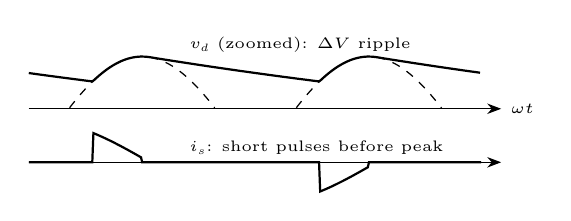
\begin{tikzpicture}[baseline=(current bounding box.south),x=9.6mm,y=3.4mm,font=\fontsize{5.5}{6}\selectfont,line width=0.45pt,>=Stealth]
\draw[->,black] (0,0)--(6.25,0) node[right,black]{$\omega t$};
\draw[dashed,black] plot coordinates{(0.541,0.039) (0.571,0.147) (0.601,0.253) (0.631,0.357) (0.661,0.458) (0.691,0.556) (0.721,0.652) (0.751,0.745) (0.781,0.835) (0.811,0.922) (0.841,1.006) (0.871,1.087) (0.901,1.165) (0.931,1.239) (0.961,1.310) (0.991,1.378) (1.021,1.442) (1.051,1.503) (1.081,1.559) (1.111,1.613) (1.141,1.662) (1.171,1.708) (1.201,1.750) (1.231,1.788) (1.261,1.822) (1.291,1.852) (1.321,1.878) (1.351,1.900) (1.381,1.918) (1.411,1.932) (1.441,1.942) (1.471,1.948) (1.501,1.950) (1.531,1.948) (1.561,1.942) (1.591,1.931) (1.621,1.917) (1.651,1.898) (1.681,1.876) (1.711,1.850) (1.741,1.819) (1.771,1.785) (1.801,1.747) (1.831,1.704) (1.861,1.658) (1.891,1.609) (1.921,1.555) (1.951,1.498) (1.981,1.437) (2.011,1.373) (2.041,1.305) (2.071,1.234) (2.101,1.159) (2.131,1.081) (2.161,1.000) (2.191,0.916) (2.221,0.828) (2.251,0.738) (2.281,0.645) (2.311,0.549) (2.341,0.450) (2.371,0.349) (2.401,0.245) (2.431,0.139) (2.461,0.031)};\draw[dashed,black] plot coordinates{(3.541,0.040) (3.571,0.148) (3.601,0.254) (3.631,0.358) (3.661,0.459) (3.691,0.557) (3.721,0.653) (3.751,0.746) (3.781,0.836) (3.811,0.923) (3.841,1.007) (3.871,1.088) (3.901,1.166) (3.931,1.240) (3.961,1.311) (3.991,1.378) (4.021,1.443) (4.051,1.503) (4.081,1.560) (4.111,1.613) (4.141,1.662) (4.171,1.708) (4.201,1.750) (4.231,1.788) (4.261,1.822) (4.291,1.852) (4.321,1.878) (4.351,1.900) (4.381,1.918) (4.411,1.932) (4.441,1.942) (4.471,1.948) (4.501,1.950) (4.531,1.948) (4.561,1.941) (4.591,1.931) (4.621,1.917) (4.651,1.898) (4.681,1.876) (4.711,1.849) (4.741,1.819) (4.771,1.785) (4.801,1.746) (4.831,1.704) (4.861,1.658) (4.891,1.608) (4.921,1.555) (4.951,1.498) (4.981,1.437) (5.011,1.372) (5.041,1.305) (5.071,1.233) (5.101,1.159) (5.131,1.081) (5.161,0.999) (5.191,0.915) (5.221,0.828) (5.251,0.737) (5.281,0.644) (5.311,0.548) (5.341,0.450) (5.371,0.348) (5.401,0.245) (5.431,0.138) (5.461,0.030)};
\draw[thick] plot coordinates{(0.001,1.334) (0.031,1.323) (0.061,1.311) (0.091,1.299) (0.121,1.288) (0.151,1.276) (0.181,1.265) (0.211,1.253) (0.241,1.242) (0.271,1.230) (0.301,1.219) (0.331,1.208) (0.361,1.197) (0.391,1.185) (0.421,1.174) (0.451,1.163) (0.481,1.152) (0.511,1.141) (0.541,1.130) (0.571,1.119) (0.601,1.108) (0.631,1.097) (0.661,1.086) (0.691,1.075) (0.721,1.064) (0.751,1.053) (0.781,1.042) (0.811,1.032) (0.841,1.021) (0.871,1.087) (0.901,1.165) (0.931,1.239) (0.961,1.310) (0.991,1.378) (1.021,1.442) (1.051,1.503) (1.081,1.559) (1.111,1.613) (1.141,1.662) (1.171,1.708) (1.201,1.750) (1.231,1.788) (1.261,1.822) (1.291,1.852) (1.321,1.878) (1.351,1.900) (1.381,1.918) (1.411,1.932) (1.441,1.942) (1.471,1.948) (1.501,1.949) (1.531,1.947) (1.561,1.941) (1.591,1.931) (1.621,1.918) (1.651,1.904) (1.681,1.890) (1.711,1.877) (1.741,1.863) (1.771,1.850) (1.801,1.836) (1.831,1.823) (1.861,1.810) (1.891,1.796) (1.921,1.783) (1.951,1.770) (1.981,1.757) (2.011,1.744) (2.041,1.731) (2.071,1.718) (2.101,1.705) (2.131,1.692) (2.161,1.679) (2.191,1.666) (2.221,1.653) (2.251,1.640) (2.281,1.627) (2.311,1.615) (2.341,1.602) (2.371,1.590) (2.401,1.577) (2.431,1.564) (2.461,1.552) (2.491,1.540) (2.521,1.527) (2.551,1.515) (2.581,1.503) (2.611,1.490) (2.641,1.478) (2.671,1.466) (2.701,1.454) (2.731,1.442) (2.761,1.429) (2.791,1.417) (2.821,1.405) (2.851,1.394) (2.881,1.382) (2.911,1.370) (2.941,1.358) (2.971,1.346) (3.001,1.334) (3.031,1.323) (3.061,1.311) (3.091,1.299) (3.121,1.288) (3.151,1.276) (3.181,1.265) (3.211,1.253) (3.241,1.242) (3.271,1.230) (3.301,1.219) (3.331,1.208) (3.361,1.196) (3.391,1.185) (3.421,1.174) (3.451,1.163) (3.481,1.152) (3.511,1.141) (3.541,1.129) (3.571,1.118) (3.601,1.107) (3.631,1.097) (3.661,1.086) (3.691,1.075) (3.721,1.064) (3.751,1.053) (3.781,1.042) (3.811,1.032) (3.841,1.021) (3.871,1.088) (3.901,1.166) (3.931,1.240) (3.961,1.311) (3.991,1.378) (4.021,1.443) (4.051,1.503) (4.081,1.560) (4.111,1.613) (4.141,1.662) (4.171,1.708) (4.201,1.750) (4.231,1.788) (4.261,1.822) (4.291,1.852) (4.321,1.878) (4.351,1.900) (4.381,1.918) (4.411,1.932) (4.441,1.942) (4.471,1.948) (4.501,1.949) (4.531,1.947) (4.561,1.941) (4.591,1.931) (4.621,1.918) (4.651,1.904) (4.681,1.890) (4.711,1.877) (4.741,1.863) (4.771,1.850) (4.801,1.836) (4.831,1.823) (4.861,1.810) (4.891,1.796) (4.921,1.783) (4.951,1.770) (4.981,1.757) (5.011,1.744) (5.041,1.730) (5.071,1.717) (5.101,1.704) (5.131,1.691) (5.161,1.679) (5.191,1.666) (5.221,1.653) (5.251,1.640) (5.281,1.627) (5.311,1.615) (5.341,1.602) (5.371,1.589) (5.401,1.577) (5.431,1.564) (5.461,1.552) (5.491,1.539) (5.521,1.527) (5.551,1.515) (5.581,1.502) (5.611,1.490) (5.641,1.478) (5.671,1.466) (5.701,1.454) (5.731,1.441) (5.761,1.429) (5.791,1.417) (5.821,1.405) (5.851,1.393) (5.881,1.382) (5.911,1.370) (5.941,1.358) (5.971,1.346)};
\draw[->,black] (0,-2.0)--(6.25,-2.0) node[right,black]{};
\draw[thick,black] plot coordinates{(0.001,-2.000) (0.016,-2.000) (0.031,-2.000) (0.046,-2.000) (0.061,-2.000) (0.076,-2.000) (0.091,-2.000) (0.106,-2.000) (0.121,-2.000) (0.136,-2.000) (0.151,-2.000) (0.166,-2.000) (0.181,-2.000) (0.196,-2.000) (0.211,-2.000) (0.226,-2.000) (0.241,-2.000) (0.256,-2.000) (0.271,-2.000) (0.286,-2.000) (0.301,-2.000) (0.316,-2.000) (0.331,-2.000) (0.346,-2.000) (0.361,-2.000) (0.376,-2.000) (0.391,-2.000) (0.406,-2.000) (0.421,-2.000) (0.436,-2.000) (0.451,-2.000) (0.466,-2.000) (0.481,-2.000) (0.496,-2.000) (0.511,-2.000) (0.526,-2.000) (0.541,-2.000) (0.556,-2.000) (0.571,-2.000) (0.586,-2.000) (0.601,-2.000) (0.616,-2.000) (0.631,-2.000) (0.646,-2.000) (0.661,-2.000) (0.676,-2.000) (0.691,-2.000) (0.706,-2.000) (0.721,-2.000) (0.736,-2.000) (0.751,-2.000) (0.766,-2.000) (0.781,-2.000) (0.796,-2.000) (0.811,-2.000) (0.826,-2.000) (0.841,-2.000) (0.856,-0.910) (0.871,-0.928) (0.886,-0.945) (0.901,-0.963) (0.916,-0.982) (0.931,-1.000) (0.946,-1.019) (0.961,-1.038) (0.976,-1.057) (0.991,-1.076) (1.006,-1.096) (1.021,-1.116) (1.036,-1.136) (1.051,-1.156) (1.066,-1.177) (1.081,-1.197) (1.096,-1.218) (1.111,-1.239) (1.126,-1.261) (1.141,-1.282) (1.156,-1.304) (1.171,-1.326) (1.186,-1.348) (1.201,-1.370) (1.216,-1.392) (1.231,-1.415) (1.246,-1.437) (1.261,-1.460) (1.276,-1.483) (1.291,-1.506) (1.306,-1.529) (1.321,-1.552) (1.336,-1.576) (1.351,-1.599) (1.366,-1.623) (1.381,-1.646) (1.396,-1.670) (1.411,-1.694) (1.426,-1.718) (1.441,-1.742) (1.456,-1.766) (1.471,-1.790) (1.486,-1.814) (1.501,-2.000) (1.516,-2.000) (1.531,-2.000) (1.546,-2.000) (1.561,-2.000) (1.576,-2.000) (1.591,-2.000) (1.606,-2.000) (1.621,-2.000) (1.636,-2.000) (1.651,-2.000) (1.666,-2.000) (1.681,-2.000) (1.696,-2.000) (1.711,-2.000) (1.726,-2.000) (1.741,-2.000) (1.756,-2.000) (1.771,-2.000) (1.786,-2.000) (1.801,-2.000) (1.816,-2.000) (1.831,-2.000) (1.846,-2.000) (1.861,-2.000) (1.876,-2.000) (1.891,-2.000) (1.906,-2.000) (1.921,-2.000) (1.936,-2.000) (1.951,-2.000) (1.966,-2.000) (1.981,-2.000) (1.996,-2.000) (2.011,-2.000) (2.026,-2.000) (2.041,-2.000) (2.056,-2.000) (2.071,-2.000) (2.086,-2.000) (2.101,-2.000) (2.116,-2.000) (2.131,-2.000) (2.146,-2.000) (2.161,-2.000) (2.176,-2.000) (2.191,-2.000) (2.206,-2.000) (2.221,-2.000) (2.236,-2.000) (2.251,-2.000) (2.266,-2.000) (2.281,-2.000) (2.296,-2.000) (2.311,-2.000) (2.326,-2.000) (2.341,-2.000) (2.356,-2.000) (2.371,-2.000) (2.386,-2.000) (2.401,-2.000) (2.416,-2.000) (2.431,-2.000) (2.446,-2.000) (2.461,-2.000) (2.476,-2.000) (2.491,-2.000) (2.506,-2.000) (2.521,-2.000) (2.536,-2.000) (2.551,-2.000) (2.566,-2.000) (2.581,-2.000) (2.596,-2.000) (2.611,-2.000) (2.626,-2.000) (2.641,-2.000) (2.656,-2.000) (2.671,-2.000) (2.686,-2.000) (2.701,-2.000) (2.716,-2.000) (2.731,-2.000) (2.746,-2.000) (2.761,-2.000) (2.776,-2.000) (2.791,-2.000) (2.806,-2.000) (2.821,-2.000) (2.836,-2.000) (2.851,-2.000) (2.866,-2.000) (2.881,-2.000) (2.896,-2.000) (2.911,-2.000) (2.926,-2.000) (2.941,-2.000) (2.956,-2.000) (2.971,-2.000) (2.986,-2.000) (3.001,-2.000) (3.016,-2.000) (3.031,-2.000) (3.046,-2.000) (3.061,-2.000) (3.076,-2.000) (3.091,-2.000) (3.106,-2.000) (3.121,-2.000) (3.136,-2.000) (3.151,-2.000) (3.166,-2.000) (3.181,-2.000) (3.196,-2.000) (3.211,-2.000) (3.226,-2.000) (3.241,-2.000) (3.256,-2.000) (3.271,-2.000) (3.286,-2.000) (3.301,-2.000) (3.316,-2.000) (3.331,-2.000) (3.346,-2.000) (3.361,-2.000) (3.376,-2.000) (3.391,-2.000) (3.406,-2.000) (3.421,-2.000) (3.436,-2.000) (3.451,-2.000) (3.466,-2.000) (3.481,-2.000) (3.496,-2.000) (3.511,-2.000) (3.526,-2.000) (3.541,-2.000) (3.556,-2.000) (3.571,-2.000) (3.586,-2.000) (3.601,-2.000) (3.616,-2.000) (3.631,-2.000) (3.646,-2.000) (3.661,-2.000) (3.676,-2.000) (3.691,-2.000) (3.706,-2.000) (3.721,-2.000) (3.736,-2.000) (3.751,-2.000) (3.766,-2.000) (3.781,-2.000) (3.796,-2.000) (3.811,-2.000) (3.826,-2.000) (3.841,-2.000) (3.856,-3.089) (3.871,-3.072) (3.886,-3.054) (3.901,-3.036) (3.916,-3.018) (3.931,-3.000) (3.946,-2.981) (3.961,-2.962) (3.976,-2.943) (3.991,-2.923) (4.006,-2.904) (4.021,-2.884) (4.036,-2.864) (4.051,-2.843) (4.066,-2.823) (4.081,-2.802) (4.096,-2.781) (4.111,-2.760) (4.126,-2.739) (4.141,-2.717) (4.156,-2.696) (4.171,-2.674) (4.186,-2.652) (4.201,-2.630) (4.216,-2.607) (4.231,-2.585) (4.246,-2.562) (4.261,-2.540) (4.276,-2.517) (4.291,-2.494) (4.306,-2.471) (4.321,-2.447) (4.336,-2.424) (4.351,-2.401) (4.366,-2.377) (4.381,-2.353) (4.396,-2.330) (4.411,-2.306) (4.426,-2.282) (4.441,-2.258) (4.456,-2.234) (4.471,-2.210) (4.486,-2.186) (4.501,-2.000) (4.516,-2.000) (4.531,-2.000) (4.546,-2.000) (4.561,-2.000) (4.576,-2.000) (4.591,-2.000) (4.606,-2.000) (4.621,-2.000) (4.636,-2.000) (4.651,-2.000) (4.666,-2.000) (4.681,-2.000) (4.696,-2.000) (4.711,-2.000) (4.726,-2.000) (4.741,-2.000) (4.756,-2.000) (4.771,-2.000) (4.786,-2.000) (4.801,-2.000) (4.816,-2.000) (4.831,-2.000) (4.846,-2.000) (4.861,-2.000) (4.876,-2.000) (4.891,-2.000) (4.906,-2.000) (4.921,-2.000) (4.936,-2.000) (4.951,-2.000) (4.966,-2.000) (4.981,-2.000) (4.996,-2.000) (5.011,-2.000) (5.026,-2.000) (5.041,-2.000) (5.056,-2.000) (5.071,-2.000) (5.086,-2.000) (5.101,-2.000) (5.116,-2.000) (5.131,-2.000) (5.146,-2.000) (5.161,-2.000) (5.176,-2.000) (5.191,-2.000) (5.206,-2.000) (5.221,-2.000) (5.236,-2.000) (5.251,-2.000) (5.266,-2.000) (5.281,-2.000) (5.296,-2.000) (5.311,-2.000) (5.326,-2.000) (5.341,-2.000) (5.356,-2.000) (5.371,-2.000) (5.386,-2.000) (5.401,-2.000) (5.416,-2.000) (5.431,-2.000) (5.446,-2.000) (5.461,-2.000) (5.476,-2.000) (5.491,-2.000) (5.506,-2.000) (5.521,-2.000) (5.536,-2.000) (5.551,-2.000) (5.566,-2.000) (5.581,-2.000) (5.596,-2.000) (5.611,-2.000) (5.626,-2.000) (5.641,-2.000) (5.656,-2.000) (5.671,-2.000) (5.686,-2.000) (5.701,-2.000) (5.716,-2.000) (5.731,-2.000) (5.746,-2.000) (5.761,-2.000) (5.776,-2.000) (5.791,-2.000) (5.806,-2.000) (5.821,-2.000) (5.836,-2.000) (5.851,-2.000) (5.866,-2.000) (5.881,-2.000) (5.896,-2.000) (5.911,-2.000) (5.926,-2.000) (5.941,-2.000) (5.956,-2.000) (5.971,-2.000) (5.986,-2.000)};
\node[anchor=west] at (2.0,2.4){$v_d$ (zoomed): $\Delta V$ ripple}; \node[anchor=west,black] at (2.0,-1.45){$i_s$: short pulses before peak};
\end{tikzpicture}\par

%=========================================================
\hd{Three-Phase Diode Rectifiers}
\nt{$V_{LL}$: rms line-to-line, $V_{ph}$: rms phase}\\
\sh{Half-wave (3 diodes, neutral)} $V_d=1.17V_{ph}$\\
\sh{Full bridge (6 diodes)} $V_d=\frac{3\sqrt2}{\pi}V_{LL}=1.35V_{LL}$\\
$v_d$ between $1.225V_{LL}$ and $1.414V_{LL}$ (6 pulses/cycle)\\
If $I_d$ constant: $i_a=\pm I_d$ for $120^\circ$\\
$I_s=0.816I_d$, $I_{s1}=0.78I_d$, $I_{sh}=I_{s1}/h$ ($h$=5,7,11,13..)\\
PF $=0.955$, THD $=31\%$\\
\sh{With $L_s$} $V_d=1.35V_{LL}-\dfrac{3\omega L_sI_d}{\pi}$, $\cos u=1-\dfrac{2\omega L_sI_d}{\sqrt2V_{LL}}$

\par\noindent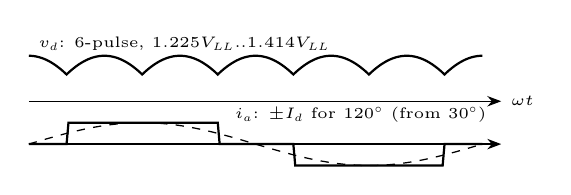
\begin{tikzpicture}[baseline=(current bounding box.south),x=9.6mm,y=3.4mm,font=\fontsize{5.5}{6}\selectfont,line width=0.45pt,>=Stealth]
\draw[->,black] (0,0)--(6.25,0) node[right,black]{$\omega t$};
\draw[thick] plot coordinates{(0.000,1.700) (0.025,1.698) (0.050,1.693) (0.075,1.684) (0.100,1.671) (0.125,1.655) (0.150,1.636) (0.175,1.613) (0.200,1.586) (0.225,1.556) (0.250,1.522) (0.275,1.485) (0.300,1.444) (0.325,1.400) (0.350,1.353) (0.375,1.302) (0.400,1.248) (0.425,1.191) (0.450,1.131) (0.475,1.067) (0.500,1.000) (0.525,1.067) (0.550,1.131) (0.575,1.191) (0.600,1.248) (0.625,1.302) (0.650,1.353) (0.675,1.400) (0.700,1.444) (0.725,1.485) (0.750,1.522) (0.775,1.556) (0.800,1.586) (0.825,1.613) (0.850,1.636) (0.875,1.655) (0.900,1.671) (0.925,1.684) (0.950,1.693) (0.975,1.698) (1.000,1.700) (1.025,1.698) (1.050,1.693) (1.075,1.684) (1.100,1.671) (1.125,1.655) (1.150,1.636) (1.175,1.613) (1.200,1.586) (1.225,1.556) (1.250,1.522) (1.275,1.485) (1.300,1.444) (1.325,1.400) (1.350,1.353) (1.375,1.302) (1.400,1.248) (1.425,1.191) (1.450,1.131) (1.475,1.067) (1.500,1.000) (1.525,1.067) (1.550,1.131) (1.575,1.191) (1.600,1.248) (1.625,1.302) (1.650,1.353) (1.675,1.400) (1.700,1.444) (1.725,1.485) (1.750,1.522) (1.775,1.556) (1.800,1.586) (1.825,1.613) (1.850,1.636) (1.875,1.655) (1.900,1.671) (1.925,1.684) (1.950,1.693) (1.975,1.698) (2.000,1.700) (2.025,1.698) (2.050,1.693) (2.075,1.684) (2.100,1.671) (2.125,1.655) (2.150,1.636) (2.175,1.613) (2.200,1.586) (2.225,1.556) (2.250,1.522) (2.275,1.485) (2.300,1.444) (2.325,1.400) (2.350,1.353) (2.375,1.302) (2.400,1.248) (2.425,1.191) (2.450,1.131) (2.475,1.067) (2.500,1.000) (2.525,1.067) (2.550,1.131) (2.575,1.191) (2.600,1.248) (2.625,1.302) (2.650,1.353) (2.675,1.400) (2.700,1.444) (2.725,1.485) (2.750,1.522) (2.775,1.556) (2.800,1.586) (2.825,1.613) (2.850,1.636) (2.875,1.655) (2.900,1.671) (2.925,1.684) (2.950,1.693) (2.975,1.698) (3.000,1.700) (3.025,1.698) (3.050,1.693) (3.075,1.684) (3.100,1.671) (3.125,1.655) (3.150,1.636) (3.175,1.613) (3.200,1.586) (3.225,1.556) (3.250,1.522) (3.275,1.485) (3.300,1.444) (3.325,1.400) (3.350,1.353) (3.375,1.302) (3.400,1.248) (3.425,1.191) (3.450,1.131) (3.475,1.067) (3.500,1.000) (3.525,1.067) (3.550,1.131) (3.575,1.191) (3.600,1.248) (3.625,1.302) (3.650,1.353) (3.675,1.400) (3.700,1.444) (3.725,1.485) (3.750,1.522) (3.775,1.556) (3.800,1.586) (3.825,1.613) (3.850,1.636) (3.875,1.655) (3.900,1.671) (3.925,1.684) (3.950,1.693) (3.975,1.698) (4.000,1.700) (4.025,1.698) (4.050,1.693) (4.075,1.684) (4.100,1.671) (4.125,1.655) (4.150,1.636) (4.175,1.613) (4.200,1.586) (4.225,1.556) (4.250,1.522) (4.275,1.485) (4.300,1.444) (4.325,1.400) (4.350,1.353) (4.375,1.302) (4.400,1.248) (4.425,1.191) (4.450,1.131) (4.475,1.067) (4.500,1.000) (4.525,1.067) (4.550,1.131) (4.575,1.191) (4.600,1.248) (4.625,1.302) (4.650,1.353) (4.675,1.400) (4.700,1.444) (4.725,1.485) (4.750,1.522) (4.775,1.556) (4.800,1.586) (4.825,1.613) (4.850,1.636) (4.875,1.655) (4.900,1.671) (4.925,1.684) (4.950,1.693) (4.975,1.698) (5.000,1.700) (5.025,1.698) (5.050,1.693) (5.075,1.684) (5.100,1.671) (5.125,1.655) (5.150,1.636) (5.175,1.613) (5.200,1.586) (5.225,1.556) (5.250,1.522) (5.275,1.485) (5.300,1.444) (5.325,1.400) (5.350,1.353) (5.375,1.302) (5.400,1.248) (5.425,1.191) (5.450,1.131) (5.475,1.067) (5.500,1.000) (5.525,1.067) (5.550,1.131) (5.575,1.191) (5.600,1.248) (5.625,1.302) (5.650,1.353) (5.675,1.400) (5.700,1.444) (5.725,1.485) (5.750,1.522) (5.775,1.556) (5.800,1.586) (5.825,1.613) (5.850,1.636) (5.875,1.655) (5.900,1.671) (5.925,1.684) (5.950,1.693) (5.975,1.698) (6.000,1.700)};
\draw[dashed,black] plot coordinates{(0.000,-1.600) (0.025,-1.579) (0.050,-1.558) (0.075,-1.537) (0.100,-1.516) (0.125,-1.496) (0.150,-1.475) (0.175,-1.454) (0.200,-1.434) (0.225,-1.413) (0.250,-1.393) (0.275,-1.373) (0.300,-1.353) (0.325,-1.333) (0.350,-1.313) (0.375,-1.294) (0.400,-1.275) (0.425,-1.256) (0.450,-1.237) (0.475,-1.218) (0.500,-1.200) (0.525,-1.182) (0.550,-1.164) (0.575,-1.147) (0.600,-1.130) (0.625,-1.113) (0.650,-1.097) (0.675,-1.080) (0.700,-1.065) (0.725,-1.049) (0.750,-1.034) (0.775,-1.020) (0.800,-1.005) (0.825,-0.992) (0.850,-0.978) (0.875,-0.965) (0.900,-0.953) (0.925,-0.941) (0.950,-0.929) (0.975,-0.918) (1.000,-0.907) (1.025,-0.897) (1.050,-0.887) (1.075,-0.878) (1.100,-0.869) (1.125,-0.861) (1.150,-0.853) (1.175,-0.846) (1.200,-0.839) (1.225,-0.833) (1.250,-0.827) (1.275,-0.822) (1.300,-0.817) (1.325,-0.813) (1.350,-0.810) (1.375,-0.807) (1.400,-0.804) (1.425,-0.802) (1.450,-0.801) (1.475,-0.800) (1.500,-0.800) (1.525,-0.800) (1.550,-0.801) (1.575,-0.802) (1.600,-0.804) (1.625,-0.807) (1.650,-0.810) (1.675,-0.813) (1.700,-0.817) (1.725,-0.822) (1.750,-0.827) (1.775,-0.833) (1.800,-0.839) (1.825,-0.846) (1.850,-0.853) (1.875,-0.861) (1.900,-0.869) (1.925,-0.878) (1.950,-0.887) (1.975,-0.897) (2.000,-0.907) (2.025,-0.918) (2.050,-0.929) (2.075,-0.941) (2.100,-0.953) (2.125,-0.965) (2.150,-0.978) (2.175,-0.992) (2.200,-1.005) (2.225,-1.020) (2.250,-1.034) (2.275,-1.049) (2.300,-1.065) (2.325,-1.080) (2.350,-1.097) (2.375,-1.113) (2.400,-1.130) (2.425,-1.147) (2.450,-1.164) (2.475,-1.182) (2.500,-1.200) (2.525,-1.218) (2.550,-1.237) (2.575,-1.256) (2.600,-1.275) (2.625,-1.294) (2.650,-1.313) (2.675,-1.333) (2.700,-1.353) (2.725,-1.373) (2.750,-1.393) (2.775,-1.413) (2.800,-1.434) (2.825,-1.454) (2.850,-1.475) (2.875,-1.496) (2.900,-1.516) (2.925,-1.537) (2.950,-1.558) (2.975,-1.579) (3.000,-1.600) (3.025,-1.621) (3.050,-1.642) (3.075,-1.663) (3.100,-1.684) (3.125,-1.704) (3.150,-1.725) (3.175,-1.746) (3.200,-1.766) (3.225,-1.787) (3.250,-1.807) (3.275,-1.827) (3.300,-1.847) (3.325,-1.867) (3.350,-1.887) (3.375,-1.906) (3.400,-1.925) (3.425,-1.944) (3.450,-1.963) (3.475,-1.982) (3.500,-2.000) (3.525,-2.018) (3.550,-2.036) (3.575,-2.053) (3.600,-2.070) (3.625,-2.087) (3.650,-2.103) (3.675,-2.120) (3.700,-2.135) (3.725,-2.151) (3.750,-2.166) (3.775,-2.180) (3.800,-2.195) (3.825,-2.208) (3.850,-2.222) (3.875,-2.235) (3.900,-2.247) (3.925,-2.259) (3.950,-2.271) (3.975,-2.282) (4.000,-2.293) (4.025,-2.303) (4.050,-2.313) (4.075,-2.322) (4.100,-2.331) (4.125,-2.339) (4.150,-2.347) (4.175,-2.354) (4.200,-2.361) (4.225,-2.367) (4.250,-2.373) (4.275,-2.378) (4.300,-2.383) (4.325,-2.387) (4.350,-2.390) (4.375,-2.393) (4.400,-2.396) (4.425,-2.398) (4.450,-2.399) (4.475,-2.400) (4.500,-2.400) (4.525,-2.400) (4.550,-2.399) (4.575,-2.398) (4.600,-2.396) (4.625,-2.393) (4.650,-2.390) (4.675,-2.387) (4.700,-2.383) (4.725,-2.378) (4.750,-2.373) (4.775,-2.367) (4.800,-2.361) (4.825,-2.354) (4.850,-2.347) (4.875,-2.339) (4.900,-2.331) (4.925,-2.322) (4.950,-2.313) (4.975,-2.303) (5.000,-2.293) (5.025,-2.282) (5.050,-2.271) (5.075,-2.259) (5.100,-2.247) (5.125,-2.235) (5.150,-2.222) (5.175,-2.208) (5.200,-2.195) (5.225,-2.180) (5.250,-2.166) (5.275,-2.151) (5.300,-2.135) (5.325,-2.120) (5.350,-2.103) (5.375,-2.087) (5.400,-2.070) (5.425,-2.053) (5.450,-2.036) (5.475,-2.018) (5.500,-2.000) (5.525,-1.982) (5.550,-1.963) (5.575,-1.944) (5.600,-1.925) (5.625,-1.906) (5.650,-1.887) (5.675,-1.867) (5.700,-1.847) (5.725,-1.827) (5.750,-1.807) (5.775,-1.787) (5.800,-1.766) (5.825,-1.746) (5.850,-1.725) (5.875,-1.704) (5.900,-1.684) (5.925,-1.663) (5.950,-1.642) (5.975,-1.621) (6.000,-1.600)};
\draw[thick,black] plot coordinates{(0.000,-1.600) (0.025,-1.600) (0.050,-1.600) (0.075,-1.600) (0.100,-1.600) (0.125,-1.600) (0.150,-1.600) (0.175,-1.600) (0.200,-1.600) (0.225,-1.600) (0.250,-1.600) (0.275,-1.600) (0.300,-1.600) (0.325,-1.600) (0.350,-1.600) (0.375,-1.600) (0.400,-1.600) (0.425,-1.600) (0.450,-1.600) (0.475,-1.600) (0.500,-1.600) (0.525,-0.800) (0.550,-0.800) (0.575,-0.800) (0.600,-0.800) (0.625,-0.800) (0.650,-0.800) (0.675,-0.800) (0.700,-0.800) (0.725,-0.800) (0.750,-0.800) (0.775,-0.800) (0.800,-0.800) (0.825,-0.800) (0.850,-0.800) (0.875,-0.800) (0.900,-0.800) (0.925,-0.800) (0.950,-0.800) (0.975,-0.800) (1.000,-0.800) (1.025,-0.800) (1.050,-0.800) (1.075,-0.800) (1.100,-0.800) (1.125,-0.800) (1.150,-0.800) (1.175,-0.800) (1.200,-0.800) (1.225,-0.800) (1.250,-0.800) (1.275,-0.800) (1.300,-0.800) (1.325,-0.800) (1.350,-0.800) (1.375,-0.800) (1.400,-0.800) (1.425,-0.800) (1.450,-0.800) (1.475,-0.800) (1.500,-0.800) (1.525,-0.800) (1.550,-0.800) (1.575,-0.800) (1.600,-0.800) (1.625,-0.800) (1.650,-0.800) (1.675,-0.800) (1.700,-0.800) (1.725,-0.800) (1.750,-0.800) (1.775,-0.800) (1.800,-0.800) (1.825,-0.800) (1.850,-0.800) (1.875,-0.800) (1.900,-0.800) (1.925,-0.800) (1.950,-0.800) (1.975,-0.800) (2.000,-0.800) (2.025,-0.800) (2.050,-0.800) (2.075,-0.800) (2.100,-0.800) (2.125,-0.800) (2.150,-0.800) (2.175,-0.800) (2.200,-0.800) (2.225,-0.800) (2.250,-0.800) (2.275,-0.800) (2.300,-0.800) (2.325,-0.800) (2.350,-0.800) (2.375,-0.800) (2.400,-0.800) (2.425,-0.800) (2.450,-0.800) (2.475,-0.800) (2.500,-0.800) (2.525,-1.600) (2.550,-1.600) (2.575,-1.600) (2.600,-1.600) (2.625,-1.600) (2.650,-1.600) (2.675,-1.600) (2.700,-1.600) (2.725,-1.600) (2.750,-1.600) (2.775,-1.600) (2.800,-1.600) (2.825,-1.600) (2.850,-1.600) (2.875,-1.600) (2.900,-1.600) (2.925,-1.600) (2.950,-1.600) (2.975,-1.600) (3.000,-1.600) (3.025,-1.600) (3.050,-1.600) (3.075,-1.600) (3.100,-1.600) (3.125,-1.600) (3.150,-1.600) (3.175,-1.600) (3.200,-1.600) (3.225,-1.600) (3.250,-1.600) (3.275,-1.600) (3.300,-1.600) (3.325,-1.600) (3.350,-1.600) (3.375,-1.600) (3.400,-1.600) (3.425,-1.600) (3.450,-1.600) (3.475,-1.600) (3.500,-1.600) (3.525,-2.400) (3.550,-2.400) (3.575,-2.400) (3.600,-2.400) (3.625,-2.400) (3.650,-2.400) (3.675,-2.400) (3.700,-2.400) (3.725,-2.400) (3.750,-2.400) (3.775,-2.400) (3.800,-2.400) (3.825,-2.400) (3.850,-2.400) (3.875,-2.400) (3.900,-2.400) (3.925,-2.400) (3.950,-2.400) (3.975,-2.400) (4.000,-2.400) (4.025,-2.400) (4.050,-2.400) (4.075,-2.400) (4.100,-2.400) (4.125,-2.400) (4.150,-2.400) (4.175,-2.400) (4.200,-2.400) (4.225,-2.400) (4.250,-2.400) (4.275,-2.400) (4.300,-2.400) (4.325,-2.400) (4.350,-2.400) (4.375,-2.400) (4.400,-2.400) (4.425,-2.400) (4.450,-2.400) (4.475,-2.400) (4.500,-2.400) (4.525,-2.400) (4.550,-2.400) (4.575,-2.400) (4.600,-2.400) (4.625,-2.400) (4.650,-2.400) (4.675,-2.400) (4.700,-2.400) (4.725,-2.400) (4.750,-2.400) (4.775,-2.400) (4.800,-2.400) (4.825,-2.400) (4.850,-2.400) (4.875,-2.400) (4.900,-2.400) (4.925,-2.400) (4.950,-2.400) (4.975,-2.400) (5.000,-2.400) (5.025,-2.400) (5.050,-2.400) (5.075,-2.400) (5.100,-2.400) (5.125,-2.400) (5.150,-2.400) (5.175,-2.400) (5.200,-2.400) (5.225,-2.400) (5.250,-2.400) (5.275,-2.400) (5.300,-2.400) (5.325,-2.400) (5.350,-2.400) (5.375,-2.400) (5.400,-2.400) (5.425,-2.400) (5.450,-2.400) (5.475,-2.400) (5.500,-1.600) (5.525,-1.600) (5.550,-1.600) (5.575,-1.600) (5.600,-1.600) (5.625,-1.600) (5.650,-1.600) (5.675,-1.600) (5.700,-1.600) (5.725,-1.600) (5.750,-1.600) (5.775,-1.600) (5.800,-1.600) (5.825,-1.600) (5.850,-1.600) (5.875,-1.600) (5.900,-1.600) (5.925,-1.600) (5.950,-1.600) (5.975,-1.600) (6.000,-1.600)};
\draw[->,black] (0,-1.6)--(6.25,-1.6) node[right,black]{};
\node[anchor=west] at (0,2.15){$v_d$: 6-pulse, $1.225V_{LL}$..$1.414V_{LL}$};\node[anchor=west,black] at (2.6,-0.5){$i_a$: $\pm I_d$ for $120^\circ$ (from $30^\circ$)};
\end{tikzpicture}\par
\sh{Three 1-$\phi$ rectifiers on 3-$\phi$ (Exp 2)}\\
Y with neutral: $I_N=3\sqrt{I_3^2+I_9^2+I_{15}^2+\dots}$\\
$\Delta$: line current $=\sqrt3\times$ branch harmonics, except 3,9,15.. which are 0 in the line

%=========================================================
\hd{Semiconductor Losses}
\sh{Diode / IGBT} model $v=V_0+r\,i$ ($r=\frac{\Delta V}{\Delta I}$ from two points)\\
$P_{cond}=V_0I_{avg}+r\,I_{rms}^2$\\
\sh{MOSFET} $P_{cond}=R_{DS(on)}I_{rms}^2$, \quad $R_{DS(on)}=V_{DS}/I_{DS}$\\
\sh{Switching} $P_{sw}=\frac12V_dI_of_s(t_{on}+t_{off})$\\
from datasheet: $P_{sw}=f_s(E_{on}+E_{off})\times\frac{V}{V_{test}}\times\frac{I}{I_{test}}$

%=========================================================
\hd{Buck \nt{(input $V_d$, output $V_o$, load $R$)}}
$V_o=DV_d$, \quad $I_L=I_o$, \quad $I_d=DI_o$\\
$v_L=V_d-V_o$ (switch on), $\ -V_o$ (switch off)\\
$\Delta i_L=\dfrac{(V_d-V_o)D}{Lf_s}=\dfrac{V_o(1-D)}{Lf_s}$, \quad $I_{L,max}=I_o+\frac{\Delta i_L}{2}$\\
$\dfrac{\Delta V_o}{V_o}=\dfrac{1-D}{8LCf_s^2}$\\
Switch and diode block $V_d$

\par\noindent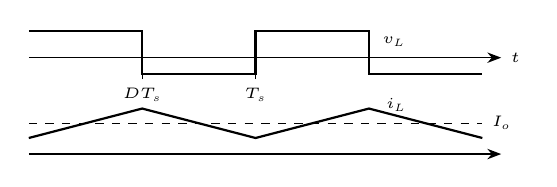
\begin{tikzpicture}[baseline=(current bounding box.south),x=9.6mm,y=3.4mm,font=\fontsize{5.5}{6}\selectfont,line width=0.45pt,>=Stealth]
\draw[->,black] (0,0)--(6.25,0) node[right,black]{$t$};
\draw[thick] (0,1.0)--(1.5,1.0)--(1.5,-0.6)--(3,-0.6)--(3,1.0)--(4.5,1.0)--(4.5,-0.6)--(6,-0.6);
\node[anchor=south west] at (4.55,0.05){$v_L$};\draw[black] (1.5,-0.6-0.2)--(1.5,-0.6+0.2); \node[black,below] at (1.5,-0.6-0.15){$DT_s$};
\draw[black] (3,-0.6-0.2)--(3,-0.6+0.2); \node[black,below] at (3,-0.6-0.15){$T_s$};
\draw[->,black] (0,-3.6)--(6.25,-3.6); \draw[thick,black] (0,-3.0)--(1.5,-1.9)--(3,-3.0)--(4.5,-1.9)--(6,-3.0); \draw[dashed] (0,-2.45)--(6,-2.45); \node[right] at (6,-2.45){$I_o$};
\node[black,anchor=west] at (4.6,-1.75){$i_L$};
\end{tikzpicture}\par

%=========================================================
\hd{Boost}
$V_o=\dfrac{V_d}{1-D}$, \quad $I_L=I_d=\dfrac{I_o}{1-D}$\\
$v_L=V_d$ (on), $\ V_d-V_o$ (off)\\
$\Delta i_L=\dfrac{V_dD}{Lf_s}$, \quad $\dfrac{\Delta V_o}{V_o}=\dfrac{D}{RCf_s}$\\
\sh{Inductor resistance $r_L$}
$\dfrac{V_o}{V_d}=\dfrac{1}{1-D}\cdot\dfrac{1}{1+\frac{r_L}{R(1-D)^2}}$\\
maximum gain $\frac12\sqrt{R/r_L}$ at $D=1-\sqrt{r_L/R}$\\
Switch and diode block $V_o$

\par\noindent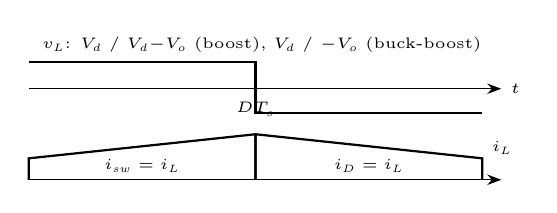
\begin{tikzpicture}[baseline=(current bounding box.south),x=9.6mm,y=3.4mm,font=\fontsize{5.5}{6}\selectfont,line width=0.45pt,>=Stealth]
\draw[->,black] (0,0)--(6.25,0) node[right,black]{$t$};
\draw[thick] (0,1.0)--(3,1.0)--(3,-0.9)--(6,-0.9);
\node[anchor=south west] at (0.05,1.0){$v_L$: $V_d$ / $V_d{-}V_o$ (boost), $V_d$ / $-V_o$ (buck-boost)};\draw[black] (3,0-0.2)--(3,0+0.2); \node[black,below] at (3,0-0.15){$DT_s$};
\draw[->,black] (0,-3.4)--(6.25,-3.4); \draw[thick,black] (0,-3.4)--(0,-2.6)--(3,-1.7)--(3,-3.4); \draw[thick,black] (3,-3.4)--(3,-1.7)--(6,-2.6)--(6,-3.4);
\node[black] at (1.5,-2.9){$i_{sw}=i_L$}; \node[black] at (4.5,-2.9){$i_D=i_L$}; \node[anchor=west] at (6,-2.2){$i_L$};
\end{tikzpicture}\par

%=========================================================
\hd{Buck-Boost \nt{(output inverted)}}
$\dfrac{V_o}{V_d}=\dfrac{D}{1-D}$, \quad $I_L=\dfrac{I_o}{1-D}$\\
$v_L=V_d$ (on), $\ -V_o$ (off)\\
$\Delta i_L=\dfrac{V_dD}{Lf_s}$, \quad $\dfrac{\Delta V_o}{V_o}=\dfrac{D}{RCf_s}$\\
Switch and diode block $V_d+V_o$\\
\sh{Interleaving} $N$ phases shifted $T_s/N$: ripple at $Nf_s$, each phase $I_o/N$

%=========================================================
\hd{Flyback}
$\dfrac{V_o}{V_s}=\dfrac{D}{1-D}\cdot\dfrac{N_2}{N_1}$\\
$v_{Lm}=V_s$ (on), $\ -V_o\frac{N_1}{N_2}$ (off)\\
avg.\ magnetizing current: $I_{Lm}=\dfrac{P_o}{V_sD}=\dfrac{V_o^2}{V_sDR}$\\
$\Delta i_{Lm}=\dfrac{V_sD}{L_mf_s}$, \quad $I_{Lm,max}=I_{Lm}+\frac{\Delta i_{Lm}}{2}$\\
diode current $=\frac{N_1}{N_2}i_{Lm}$ (off), \quad $\dfrac{\Delta V_o}{V_o}=\dfrac{D}{RCf_s}$\\
\sh{Stress} switch: $V_s+\frac{N_1}{N_2}V_o$, \quad diode: $V_o+\frac{N_2}{N_1}V_s$

\par\noindent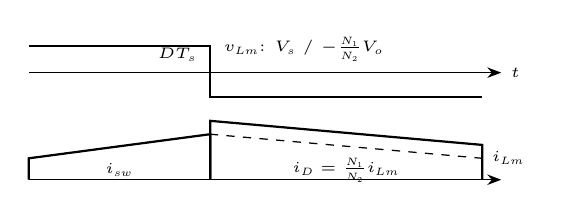
\begin{tikzpicture}[baseline=(current bounding box.south),x=9.6mm,y=3.4mm,font=\fontsize{5.5}{6}\selectfont,line width=0.45pt,>=Stealth]
\draw[->,black] (0,0)--(6.25,0) node[right,black]{$t$};
\draw[thick] (0,1.0)--(2.4,1.0)--(2.4,-0.9)--(6,-0.9);
\node[anchor=south west] at (2.45,0.05){$v_{Lm}$: $V_s$ / $-\frac{N_1}{N_2}V_o$};\node[black,anchor=south east] at (2.35,0.05){$DT_s$};
\draw[->,black] (0,-4.0)--(6.25,-4.0); \draw[dashed] (0,-3.2)--(2.4,-2.3)--(6,-3.2); \draw[thick,black] (0,-4.0)--(0,-3.2)--(2.4,-2.3)--(2.4,-4.0); \draw[thick,black] (2.4,-4.0)--(2.4,-1.8)--(6,-2.7)--(6,-4.0);
\node[black] at (1.2,-3.65){$i_{sw}$}; \node[black] at (4.2,-3.65){$i_D=\frac{N_1}{N_2}i_{Lm}$}; \node[anchor=west] at (6,-3.2){$i_{Lm}$};
\end{tikzpicture}\par

%=========================================================
\hd{Forward \nt{($N_3$: reset winding)}}
$V_o=V_sD\dfrac{N_2}{N_1}$\\
reset time $t_x=DT_s\frac{N_3}{N_1}$, \quad $D_{max}=\dfrac{1}{1+N_3/N_1}$ \nt{(0.5 if $N_3=N_1$)}\\
switch stress: $V_s\left(1+\frac{N_1}{N_3}\right)$, \quad $\Delta i_{Lm}=\dfrac{V_sD}{L_mf_s}$\\
output filter: $\Delta i_{Lx}=\dfrac{V_o(1-D)}{L_xf_s}$\\
peak switch current: $\frac{N_2}{N_1}\left(I_o+\frac{\Delta i_{Lx}}{2}\right)+\Delta i_{Lm}$

\par\noindent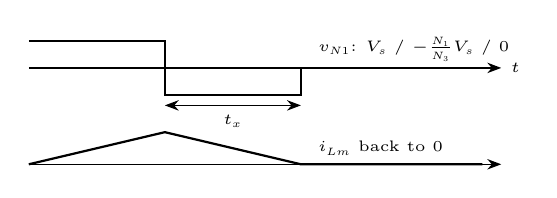
\begin{tikzpicture}[baseline=(current bounding box.south),x=9.6mm,y=3.4mm,font=\fontsize{5.5}{6}\selectfont,line width=0.45pt,>=Stealth]
\draw[->,black] (0,0)--(6.25,0) node[right,black]{$t$};
\draw[thick] (0,1.0)--(1.8,1.0)--(1.8,-1.0)--(3.6,-1.0)--(3.6,0)--(6,0);
\node[anchor=west] at (3.7,0.7){$v_{N1}$: $V_s$ / $-\frac{N_1}{N_3}V_s$ / 0}; \draw[black,<->] (1.8,-1.4)--(3.6,-1.4) node[midway,below]{$t_x$};
\draw[->,black] (0,-3.6)--(6.25,-3.6); \draw[thick,black] (0,-3.6)--(1.8,-2.4)--(3.6,-3.6)--(6,-3.6); \node[black,anchor=west] at (3.7,-3.0){$i_{Lm}$ back to 0};
\end{tikzpicture}\par

%=========================================================
\hd{Push-Pull \nt{($N_1$: each primary half)}}
$V_o=2D\dfrac{N_2}{N_1}V_s$ \quad ($D\le0.5$ for each switch)\\
switch stress: $2V_s$\\
output ripple at $2f_s$: $\Delta i_{Lx}=\dfrac{V_o(0.5-D)}{L_xf_s}$\\
switch current $\approx\frac{N_2}{N_1}I_o$ during $DT_s$

\par\noindent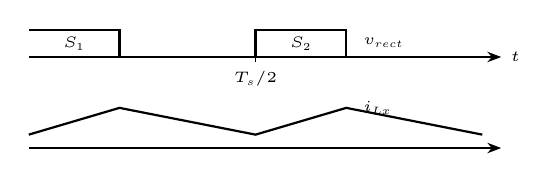
\begin{tikzpicture}[baseline=(current bounding box.south),x=9.6mm,y=3.4mm,font=\fontsize{5.5}{6}\selectfont,line width=0.45pt,>=Stealth]
\draw[->,black] (0,0)--(6.25,0) node[right,black]{$t$};
\draw[thick] (0,1.0)--(1.2,1.0)--(1.2,0)--(3,0)--(3,1.0)--(4.2,1.0)--(4.2,0)--(6,0);
\node at (0.6,0.5){$S_1$}; \node at (3.6,0.5){$S_2$}; \node[anchor=west] at (4.3,0.55){$v_{rect}$};\draw[black] (3,0-0.2)--(3,0+0.2); \node[black,below] at (3,0-0.15){$T_s/2$};
\draw[->,black] (0,-3.4)--(6.25,-3.4); \draw[thick,black] (0,-2.9)--(1.2,-1.9)--(3,-2.9)--(4.2,-1.9)--(6,-2.9);
\node[black,anchor=west] at (4.3,-1.9){$i_{Lx}$};
\end{tikzpicture}\par

%=========================================================
\hd{Inductor Design}
$\mu_0=4\pi\times10^{-7}$ H/m\\
Reluctance: $\mathcal R=\dfrac{l}{\mu_0\mu_rA}$, \quad $Ni=\phi\,\mathcal R$, \quad $B=\dfrac{\phi}{A}$\\
$L=\dfrac{N^2}{\mathcal R}=A_LN^2$ \nt{($A_L$: given in nH/turn$^2$)} $\Rightarrow N=\sqrt{L/A_L}$\\
Flux density: $B=\dfrac{L\,i}{N\,A_e}$, \quad field: $H=\dfrac{N\,i}{l_e}$\\
Min.\ turns to avoid saturation: $N\ge\dfrac{L\,I_{pk}}{B_{max}A_e}$\\
Ripple flux: $\Delta B=\dfrac{L\,\Delta i}{N\,A_e}$\\
\sh{Air gap} $L\approx\dfrac{\mu_0N^2A_e}{l_g}$ $\Rightarrow$ $l_g=\dfrac{\mu_0N^2A_e}{L}$\\
with core: $\mathcal R=\frac{l_e}{\mu_0\mu_rA_e}+\frac{l_g}{\mu_0A_e}$, \quad $l_g=\frac{\mu_0N^2A_e}{L}-\frac{l_e}{\mu_r}$\\
Energy: $E=\frac12Li^2$, \quad energy density $w=\dfrac{B^2}{2\mu_0\mu_r}$ (J/m$^3$)\\
\sh{Area product} $A_eA_w\ge\dfrac{L\,I_{pk}\,I_{rms}}{k_{cu}\,J\,B_{max}}$\\
\sh{Wire} copper area $A_{cu}=\dfrac{I_{rms}}{J}$ \nt{($J$: current density)}\\
fill factor $k_{cu}=\dfrac{N\,A_{cu}}{A_w}$ \nt{($A_w$: window area)}\\
resistance $R=\rho\dfrac{N\cdot\text{MLT}}{A_{cu}}$ \nt{(MLT: length of one turn)}\\
$n$ parallel strands: $A_{cu}=n\times A_{strand}$\\
\sh{Skin depth} $\delta=\dfrac{7.5}{\sqrt f}$ cm \nt{(copper)}; use strands with diameter $\le2\delta$\\
\sh{Losses} copper: $P_{cu}=I_{rms}^2R$\\
core (Steinmetz): $P_{fe}=k\,f^{\alpha}B^{\beta}\times$ Volume, \quad Volume $=A_el_e$

\end{multicols*}
\end{document}
